\documentclass[DIV=calc, paper=a4, fontsize=11pt]{scrartcl}\usepackage[]{graphicx}\usepackage[]{color}
%% maxwidth is the original width if it is less than linewidth
%% otherwise use linewidth (to make sure the graphics do not exceed the margin)
\makeatletter
\def\maxwidth{ %
  \ifdim\Gin@nat@width>\linewidth
    \linewidth
  \else
    \Gin@nat@width
  \fi
}
\makeatother

\definecolor{fgcolor}{rgb}{0.345, 0.345, 0.345}
\newcommand{\hlnum}[1]{\textcolor[rgb]{0.686,0.059,0.569}{#1}}%
\newcommand{\hlstr}[1]{\textcolor[rgb]{0.192,0.494,0.8}{#1}}%
\newcommand{\hlcom}[1]{\textcolor[rgb]{0.678,0.584,0.686}{\textit{#1}}}%
\newcommand{\hlopt}[1]{\textcolor[rgb]{0,0,0}{#1}}%
\newcommand{\hlstd}[1]{\textcolor[rgb]{0.345,0.345,0.345}{#1}}%
\newcommand{\hlkwa}[1]{\textcolor[rgb]{0.161,0.373,0.58}{\textbf{#1}}}%
\newcommand{\hlkwb}[1]{\textcolor[rgb]{0.69,0.353,0.396}{#1}}%
\newcommand{\hlkwc}[1]{\textcolor[rgb]{0.333,0.667,0.333}{#1}}%
\newcommand{\hlkwd}[1]{\textcolor[rgb]{0.737,0.353,0.396}{\textbf{#1}}}%

\usepackage{framed}
\makeatletter
\newenvironment{kframe}{%
 \def\at@end@of@kframe{}%
 \ifinner\ifhmode%
  \def\at@end@of@kframe{\end{minipage}}%
  \begin{minipage}{\columnwidth}%
 \fi\fi%
 \def\FrameCommand##1{\hskip\@totalleftmargin \hskip-\fboxsep
 \colorbox{shadecolor}{##1}\hskip-\fboxsep
     % There is no \\@totalrightmargin, so:
     \hskip-\linewidth \hskip-\@totalleftmargin \hskip\columnwidth}%
 \MakeFramed {\advance\hsize-\width
   \@totalleftmargin\z@ \linewidth\hsize
   \@setminipage}}%
 {\par\unskip\endMakeFramed%
 \at@end@of@kframe}
\makeatother

\definecolor{shadecolor}{rgb}{.97, .97, .97}
\definecolor{messagecolor}{rgb}{0, 0, 0}
\definecolor{warningcolor}{rgb}{1, 0, 1}
\definecolor{errorcolor}{rgb}{1, 0, 0}
\newenvironment{knitrout}{}{} % an empty environment to be redefined in TeX

\usepackage{alltt}
\usepackage[cm]{fullpage} %reduce the margin set by latex of 60-70 words per line
\usepackage{hyperref} %control links color and appearance
\hypersetup{colorlinks=true ,linkcolor=red} %setup link color to red
\usepackage[protrusion=true,expansion=true]{microtype} % Better typography
%\documentclass{scrartcl}
\usepackage{graphicx} %package for attaching images
\IfFileExists{upquote.sty}{\usepackage{upquote}}{}
\begin{document}
\title{Solution to s3.6-graph-exercise}
\author{}
\date{\today}
\maketitle{}
\clearpage
\begin{knitrout}
\definecolor{shadecolor}{rgb}{0.969, 0.969, 0.969}\color{fgcolor}\begin{kframe}
\begin{alltt}
\hlcom{# setting the working directory}


\hlcom{# load the packages}
\hlkwd{library}\hlstd{(ggplot2)}  \hlcom{#used for plotting}
\hlkwd{library}\hlstd{(foreign)}  \hlcom{#allow reading of dta files}
\hlcom{# library(reshape2)}
\hlkwd{library}\hlstd{(doBy)}  \hlcom{#provide summary of data}
\end{alltt}


{\ttfamily\noindent\itshape\color{messagecolor}{\#\# Loading required package: survival\\\#\# Loading required package: splines\\\#\# Loading required package: MASS}}\end{kframe}
\end{knitrout}

\section*{******** QUESTION 2 SOLUTION *******}

\begin{knitrout}
\definecolor{shadecolor}{rgb}{0.969, 0.969, 0.969}\color{fgcolor}\begin{kframe}
\begin{alltt}
\hlcom{# load the data set}
\hlstd{zambia3} \hlkwb{<-} \hlkwd{as.data.frame}\hlstd{(}\hlkwd{read.dta}\hlstd{(}\hlstr{"zambia3.dta"}\hlstd{,} \hlkwc{convert.dates} \hlstd{=} \hlnum{TRUE}\hlstd{))}

\hlcom{# summarize the count of data by education and urban/rural}
\hlstd{total.id} \hlkwb{<-} \hlkwd{summaryBy}\hlstd{(id} \hlopt{~} \hlstd{educ} \hlopt{+} \hlstd{urban,} \hlkwc{data} \hlstd{= zambia3,} \hlkwc{FUN} \hlstd{=} \hlkwa{function}\hlstd{(}\hlkwc{x}\hlstd{)} \hlkwd{c}\hlstd{(}\hlkwc{count} \hlstd{=} \hlkwd{length}\hlstd{(x)))}
\hlkwd{as.data.frame}\hlstd{(total.id)}
\end{alltt}
\begin{verbatim}
##                   educ urban id.count
## 1         No education     1       72
## 2         No education     2      385
## 3    Primary education     1      455
## 4    Primary education     2     1258
## 5    Primary education    NA        1
## 6  Secondary education     1      676
## 7  Secondary education     2      458
## 8  Secondary education    NA        1
## 9     Higher education     1      108
## 10    Higher education     2       29
## 11                <NA>     1       13
## 12                <NA>     2       18
\end{verbatim}
\begin{alltt}
\hlcom{# *DISTRIBUTION OF EDUCATION IN URBAN AND RURAL AREAS}
\hlkwd{ggplot}\hlstd{(total.id[}\hlopt{!}\hlkwd{is.na}\hlstd{(total.id}\hlopt{$}\hlstd{urban), ],} \hlkwd{aes}\hlstd{(}\hlkwd{as.factor}\hlstd{(urban),} \hlkwc{fill} \hlstd{= educ,}
    \hlkwc{weight} \hlstd{= id.count))} \hlopt{+} \hlkwd{geom_bar}\hlstd{(}\hlkwc{position} \hlstd{=} \hlstr{"dodge"}\hlstd{)} \hlopt{+} \hlkwd{ylab}\hlstd{(}\hlstr{"Number of respodents"}\hlstd{)} \hlopt{+}
    \hlkwd{xlab}\hlstd{(}\hlstr{""}\hlstd{)} \hlopt{+} \hlkwd{ggtitle}\hlstd{(}\hlstr{""}\hlstd{)}
\end{alltt}
\end{kframe}
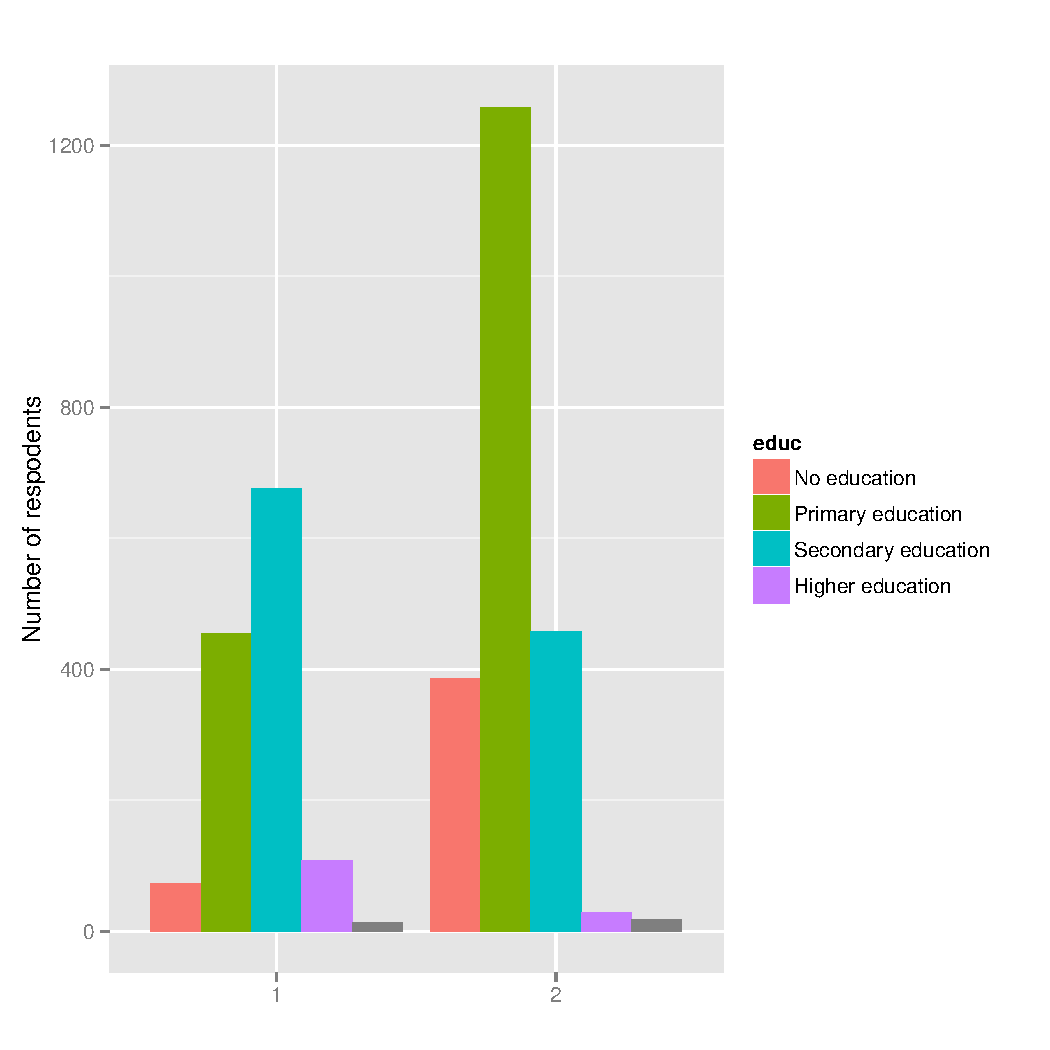
\includegraphics[width=\maxwidth]{figure/unnamed-chunk-21} 
\begin{kframe}\begin{alltt}
\hlcom{# *YOU PROBABLY WANT TO ADD A TEXT LABEL TO THE CATEGORY AXIS. *EITHER LABEL}
\hlcom{# THE URBAN VARIABLE OR:}
\hlstd{total.id}\hlopt{$}\hlstd{urban} \hlkwb{<-} \hlkwd{factor}\hlstd{(total.id}\hlopt{$}\hlstd{urban,} \hlkwc{levels} \hlstd{=} \hlkwd{c}\hlstd{(}\hlnum{1}\hlstd{,} \hlnum{2}\hlstd{),} \hlkwc{labels} \hlstd{=} \hlkwd{c}\hlstd{(}\hlstr{"Urban"}\hlstd{,}
    \hlstr{"Rural"}\hlstd{))}
\hlkwd{ggplot}\hlstd{(total.id[}\hlopt{!}\hlkwd{is.na}\hlstd{(total.id}\hlopt{$}\hlstd{urban), ],} \hlkwd{aes}\hlstd{(}\hlkwd{as.factor}\hlstd{(urban),} \hlkwc{fill} \hlstd{= educ,}
    \hlkwc{weight} \hlstd{= id.count))} \hlopt{+} \hlkwd{geom_bar}\hlstd{(}\hlkwc{position} \hlstd{=} \hlstr{"dodge"}\hlstd{)} \hlopt{+} \hlkwd{ylab}\hlstd{(}\hlstr{"Number of respodents"}\hlstd{)} \hlopt{+}
    \hlkwd{xlab}\hlstd{(}\hlstr{""}\hlstd{)} \hlopt{+} \hlkwd{ggtitle}\hlstd{(}\hlstr{""}\hlstd{)}
\end{alltt}
\end{kframe}
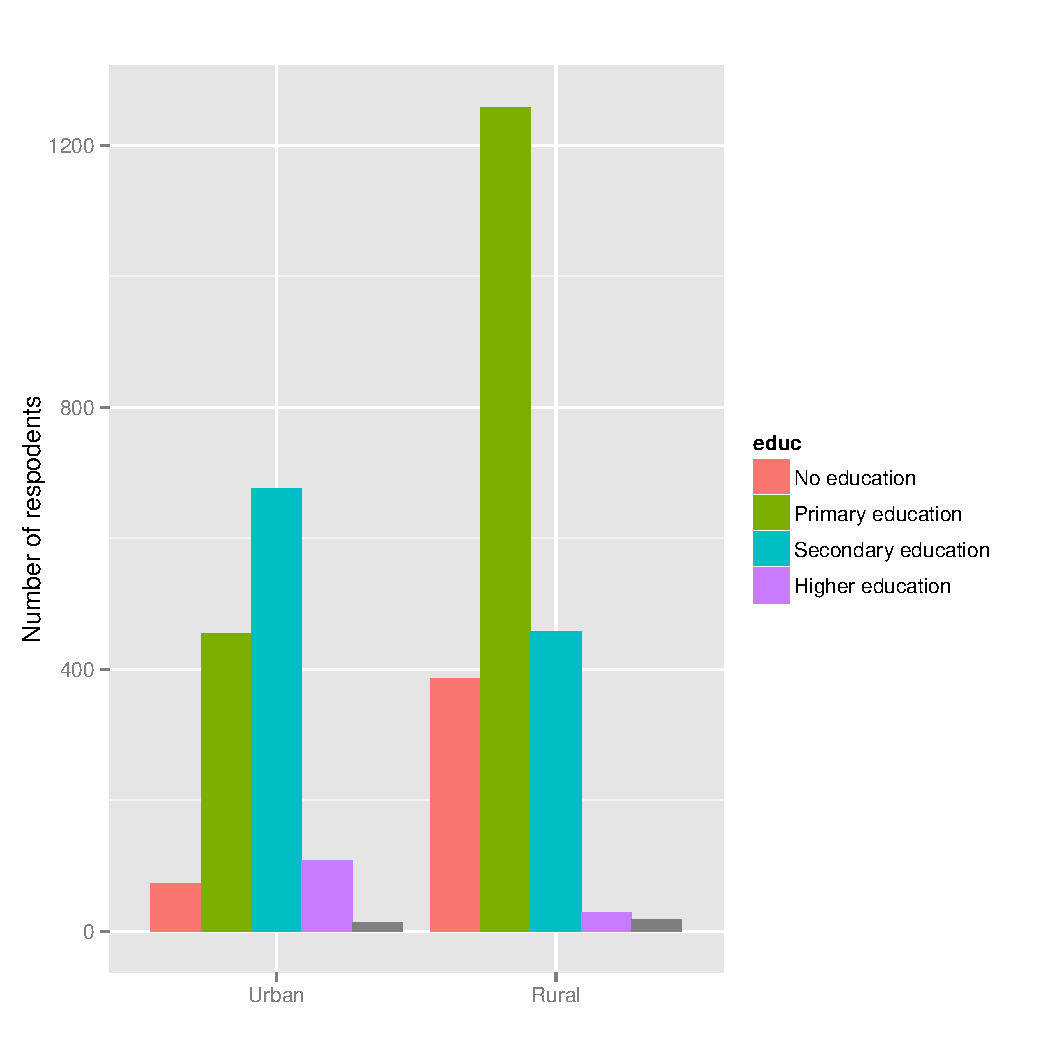
\includegraphics[width=\maxwidth]{figure/unnamed-chunk-22} 
\begin{kframe}\begin{alltt}
\hlkwd{ggsave}\hlstd{(}\hlkwc{filename} \hlstd{=} \hlstr{"gr2b4.wmf"}\hlstd{)}
\end{alltt}


{\ttfamily\noindent\itshape\color{messagecolor}{\#\# Saving 7 x 7 in image}}\begin{alltt}
\hlcom{# *WITH MOST OF THE COLOURS CHANGED}
\hlkwd{ggplot}\hlstd{(total.id[}\hlopt{!}\hlkwd{is.na}\hlstd{(total.id}\hlopt{$}\hlstd{urban), ],} \hlkwd{aes}\hlstd{(}\hlkwd{as.factor}\hlstd{(urban),} \hlkwc{fill} \hlstd{= educ,}
    \hlkwc{weight} \hlstd{= id.count))} \hlopt{+} \hlkwd{geom_bar}\hlstd{(}\hlkwc{position} \hlstd{=} \hlstr{"dodge"}\hlstd{)} \hlopt{+} \hlkwd{ylab}\hlstd{(}\hlstr{"Number of respodents"}\hlstd{)} \hlopt{+}
    \hlkwd{xlab}\hlstd{(}\hlstr{""}\hlstd{)} \hlopt{+} \hlkwd{ggtitle}\hlstd{(}\hlstr{""}\hlstd{)} \hlopt{+} \hlkwd{scale_fill_manual}\hlstd{(}\hlkwc{values} \hlstd{=} \hlkwd{c}\hlstd{(}\hlkwc{`No education`} \hlstd{=} \hlstr{"red"}\hlstd{,}
    \hlkwc{`Primary education`} \hlstd{=} \hlstr{"orange"}\hlstd{,} \hlkwc{`Secondary education`} \hlstd{=} \hlstr{"blue"}\hlstd{,} \hlkwc{`Higher education`} \hlstd{=} \hlstr{"green"}\hlstd{))} \hlopt{+}
    \hlkwd{theme}\hlstd{(}\hlkwc{panel.background} \hlstd{=} \hlkwd{element_rect}\hlstd{(}\hlkwc{fill} \hlstd{=} \hlstr{"gray"}\hlstd{),} \hlkwc{panel.grid.major} \hlstd{=} \hlkwd{element_line}\hlstd{(}\hlkwc{colour} \hlstd{=} \hlstr{"black"}\hlstd{),}
        \hlkwc{panel.grid.minor} \hlstd{=} \hlkwd{element_line}\hlstd{(}\hlkwc{colour} \hlstd{=} \hlstr{"red"}\hlstd{,} \hlkwc{linetype} \hlstd{=} \hlstr{"dotted"}\hlstd{),}
        \hlkwc{plot.background} \hlstd{=} \hlkwd{element_rect}\hlstd{(}\hlkwc{fill} \hlstd{=} \hlstr{"cyan"}\hlstd{),} \hlkwc{legend.background} \hlstd{=} \hlkwd{element_rect}\hlstd{(}\hlkwc{colour} \hlstd{=} \hlstr{"black"}\hlstd{),}
        \hlkwc{legend.key} \hlstd{=} \hlkwd{element_rect}\hlstd{(}\hlkwc{fill} \hlstd{=} \hlstr{"yellow"}\hlstd{))}
\end{alltt}
\end{kframe}
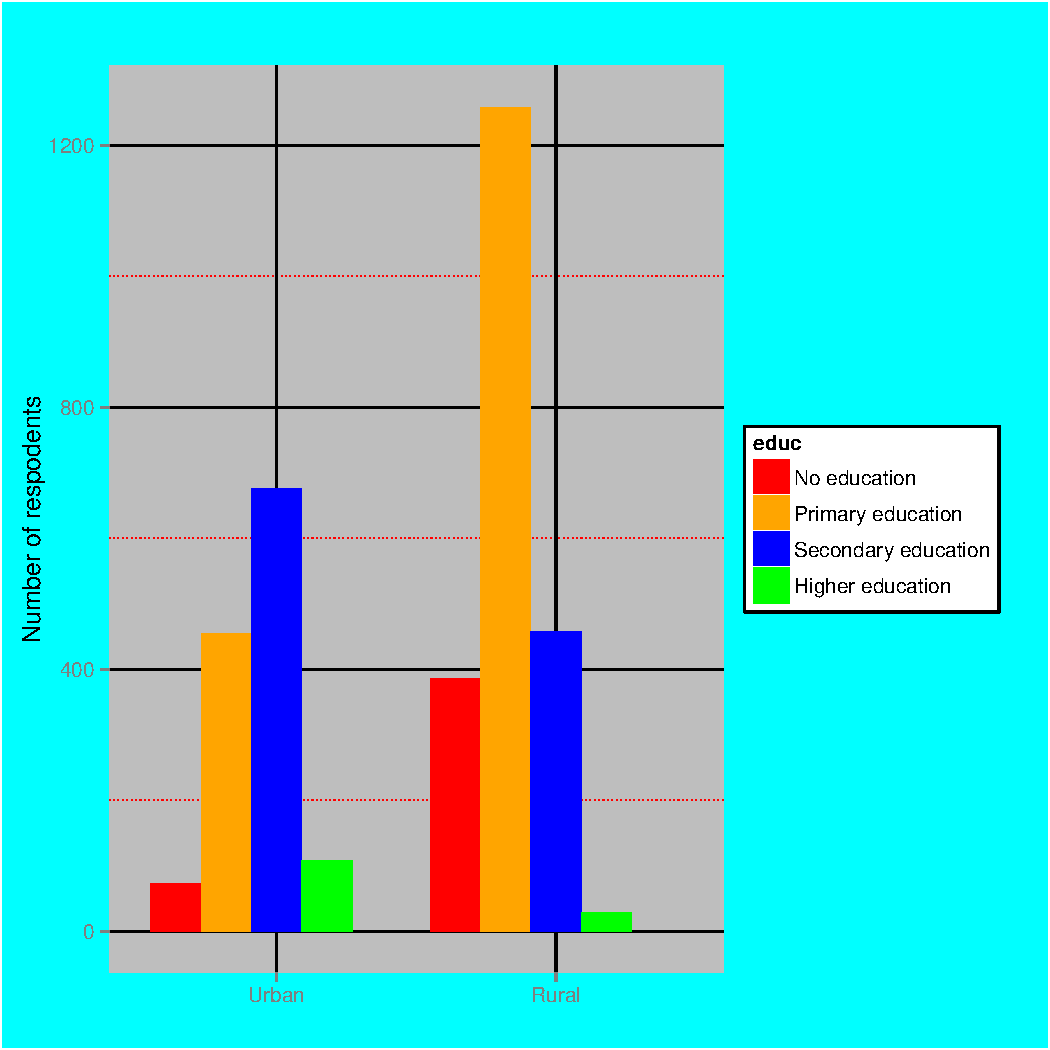
\includegraphics[width=\maxwidth]{figure/unnamed-chunk-23} 

\end{knitrout}

\section*{******** QUESTION 3 SOLUTION *******}
\begin{knitrout}
\definecolor{shadecolor}{rgb}{0.969, 0.969, 0.969}\color{fgcolor}\begin{kframe}
\begin{alltt}
\hlcom{# load the data set}
\hlstd{bab9} \hlkwb{<-} \hlkwd{as.data.frame}\hlstd{(}\hlkwd{read.dta}\hlstd{(}\hlstr{"bab9.dta"}\hlstd{,} \hlkwc{convert.dates} \hlstd{=} \hlnum{TRUE}\hlstd{))}
\hlstd{bab9} \hlkwb{<-} \hlkwd{as.data.frame}\hlstd{(bab9)}
\hlkwd{ggplot}\hlstd{(bab9,} \hlkwd{aes}\hlstd{(}\hlkwd{factor}\hlstd{(gestcat), bweight))} \hlopt{+} \hlkwd{geom_boxplot}\hlstd{()}
\end{alltt}
\end{kframe}
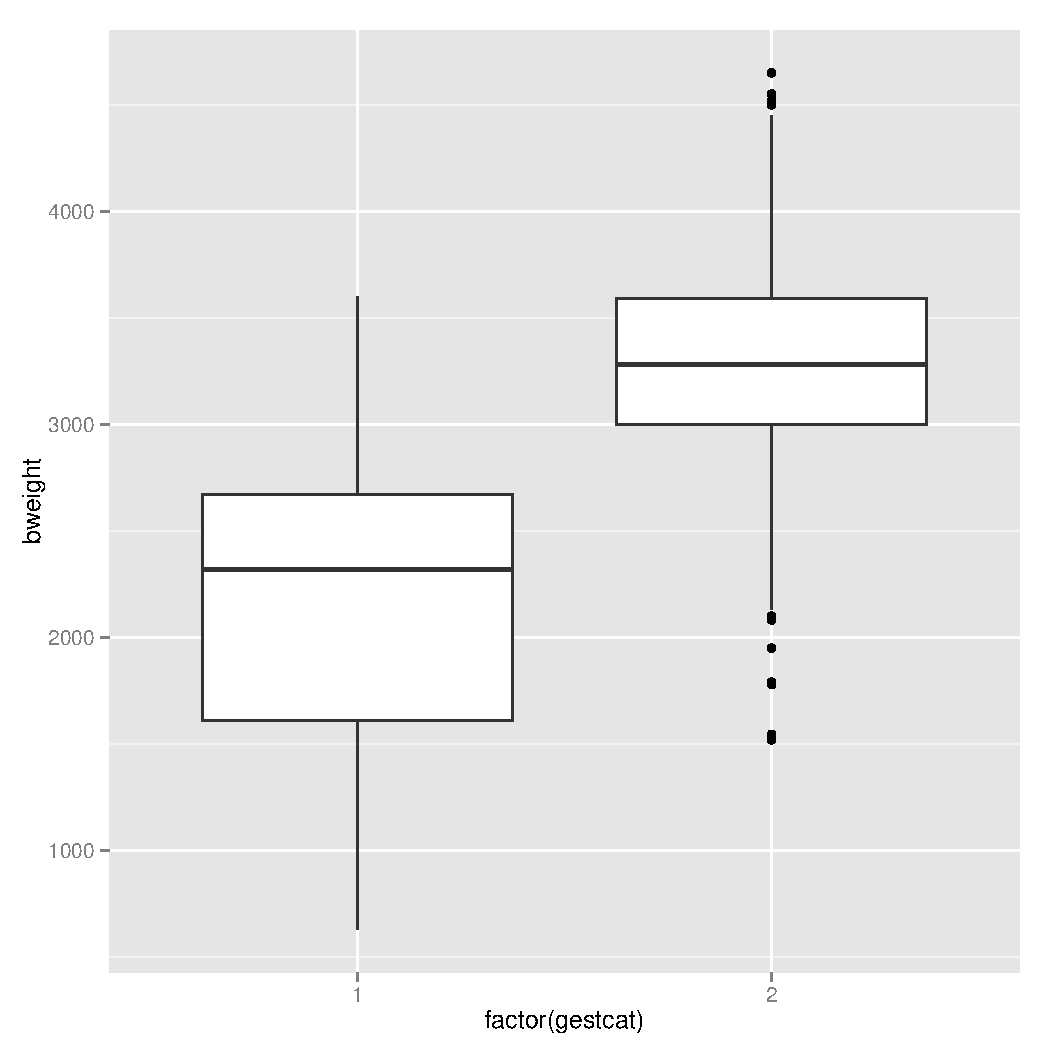
\includegraphics[width=\maxwidth]{figure/unnamed-chunk-31} 
\begin{kframe}\begin{alltt}
\hlcom{# *WITH A TITLE BELOW THE GRAPH}
\hlkwd{ggplot}\hlstd{(bab9,} \hlkwd{aes}\hlstd{(}\hlkwd{factor}\hlstd{(gestcat), bweight))} \hlopt{+} \hlkwd{geom_boxplot}\hlstd{()} \hlopt{+} \hlkwd{ggtitle}\hlstd{(}\hlstr{"Birth weight by gestational age"}\hlstd{)} \hlopt{+}
    \hlkwd{theme}\hlstd{(}\hlkwc{plot.title} \hlstd{=} \hlkwd{element_text}\hlstd{(}\hlkwc{vjust} \hlstd{=} \hlopt{-}\hlnum{54}\hlstd{))} \hlopt{+} \hlkwd{xlab}\hlstd{(}\hlstr{""}\hlstd{)}
\end{alltt}
\end{kframe}
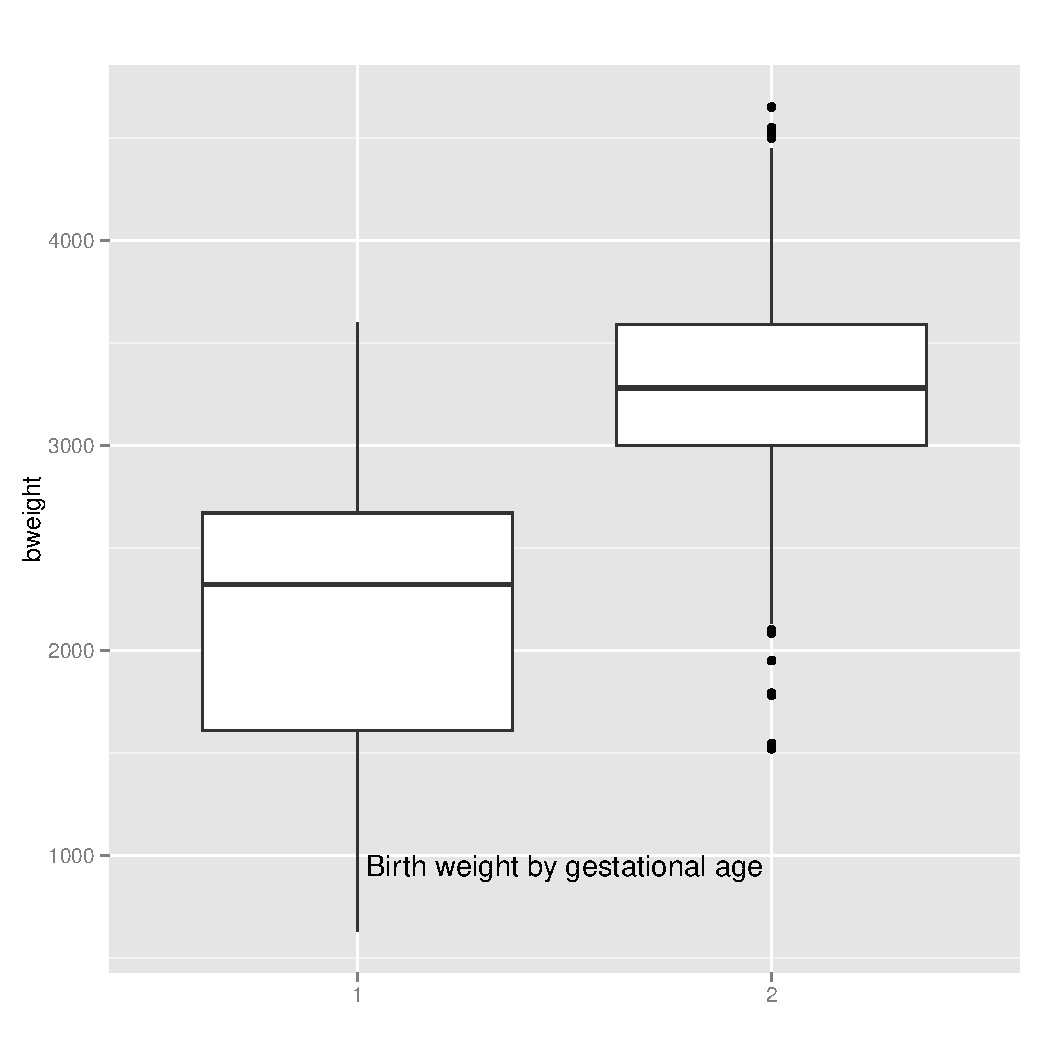
\includegraphics[width=\maxwidth]{figure/unnamed-chunk-32} 
\begin{kframe}\begin{alltt}
\hlcom{# *AGAIN YOU CAN LABEL THE gestcat VARIABLE OR WRITE YOUR *OWN LABELS ON THE}
\hlcom{# X-AXIS}
\hlstd{bab9}\hlopt{$}\hlstd{gestcat} \hlkwb{<-} \hlkwd{factor}\hlstd{(bab9}\hlopt{$}\hlstd{gestcat,} \hlkwc{levels} \hlstd{=} \hlkwd{c}\hlstd{(}\hlnum{1}\hlstd{,} \hlnum{2}\hlstd{),} \hlkwc{labels} \hlstd{=} \hlkwd{c}\hlstd{(}\hlstr{"Premature"}\hlstd{,}
    \hlstr{"Term"}\hlstd{))}
\hlkwd{ggplot}\hlstd{(bab9,} \hlkwd{aes}\hlstd{(}\hlkwd{factor}\hlstd{(gestcat), bweight))} \hlopt{+} \hlkwd{geom_boxplot}\hlstd{()} \hlopt{+} \hlkwd{ggtitle}\hlstd{(}\hlstr{"Birth weight by gestational age"}\hlstd{)} \hlopt{+}
    \hlkwd{theme}\hlstd{(}\hlkwc{plot.title} \hlstd{=} \hlkwd{element_text}\hlstd{(}\hlkwc{vjust} \hlstd{=} \hlopt{-}\hlnum{54}\hlstd{))} \hlopt{+} \hlkwd{xlab}\hlstd{(}\hlstr{""}\hlstd{)}
\end{alltt}
\end{kframe}
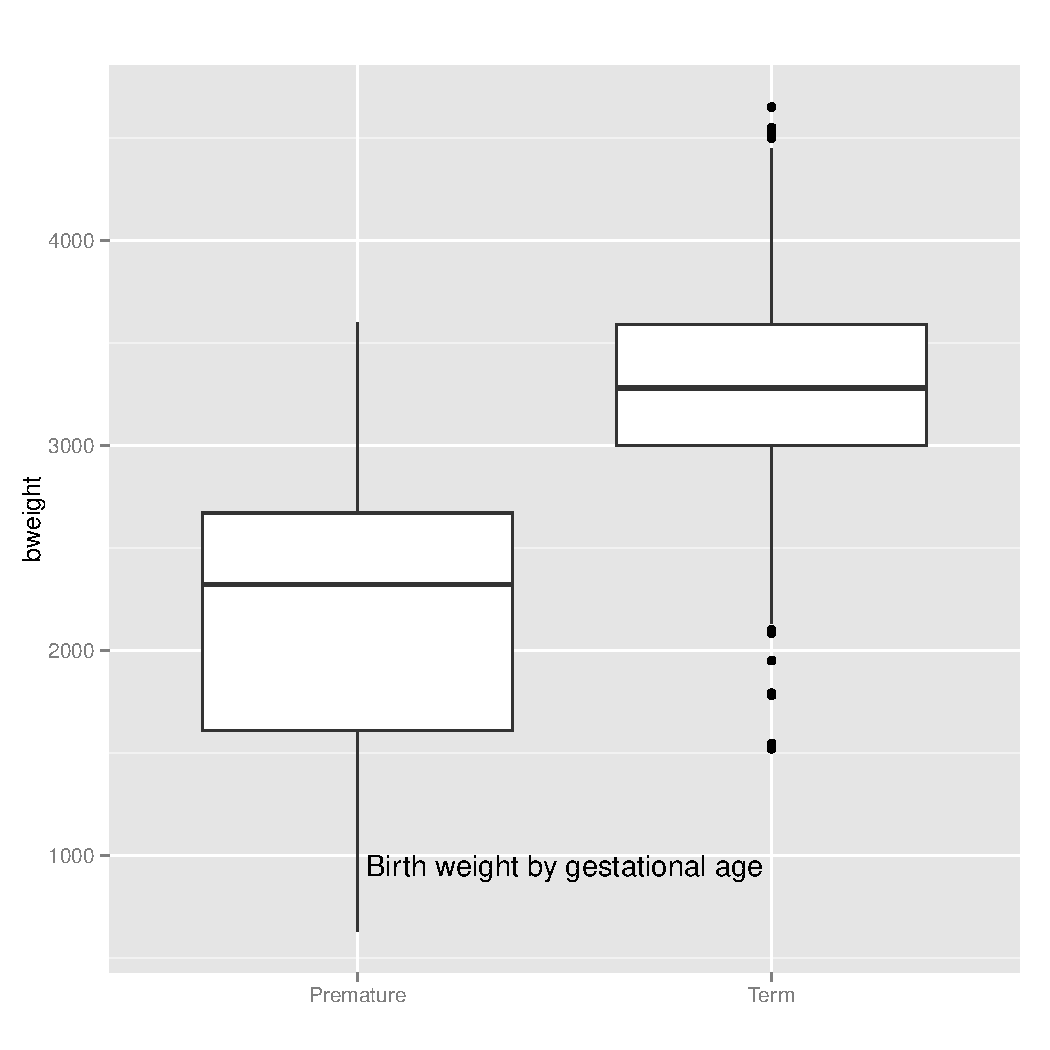
\includegraphics[width=\maxwidth]{figure/unnamed-chunk-33} 

\end{knitrout}

\section*{******** QUESTION 4 SOLUTION *******}
\begin{knitrout}
\definecolor{shadecolor}{rgb}{0.969, 0.969, 0.969}\color{fgcolor}\begin{kframe}
\begin{alltt}
\hlcom{# load the data set}
\hlstd{zambia4} \hlkwb{<-} \hlkwd{as.data.frame}\hlstd{(}\hlkwd{read.dta}\hlstd{(}\hlstr{"zambia4_isingo.dta"}\hlstd{,} \hlkwc{convert.dates} \hlstd{=} \hlnum{TRUE}\hlstd{))}
\end{alltt}


{\ttfamily\noindent\color{warningcolor}{\#\# Warning: value labels ('currmarrlbl') for 'married' are missing}}\begin{alltt}
\hlstd{zambia4} \hlkwb{<-} \hlkwd{as.data.frame}\hlstd{(zambia4)}
\hlcom{# *PIE CHART FOR EDUCATIONAL LEVEL OF WOMEN WHO USED A CONDOM *AT LAST SEX}
\hlcom{# AND THOSE WHO DID NOT summarize the count of data by education and}
\hlcom{# urban/rural}
\hlkwd{ggplot}\hlstd{(zambia4[}\hlopt{!}\hlkwd{is.na}\hlstd{(zambia4}\hlopt{$}\hlstd{clastsex), ],} \hlkwd{aes}\hlstd{(}\hlkwc{x} \hlstd{=} \hlkwd{factor}\hlstd{(}\hlnum{1}\hlstd{),} \hlkwc{fill} \hlstd{= educ,}
    \hlkwc{weight} \hlstd{= weight))} \hlopt{+} \hlkwd{coord_polar}\hlstd{(}\hlkwc{theta} \hlstd{=} \hlstr{"y"}\hlstd{)} \hlopt{+} \hlkwd{scale_x_discrete}\hlstd{(}\hlstr{""}\hlstd{)} \hlopt{+} \hlkwd{facet_grid}\hlstd{(}\hlkwc{facets} \hlstd{= .} \hlopt{~}
    \hlstd{clastsex)} \hlopt{+} \hlkwd{geom_bar}\hlstd{(}\hlkwc{width} \hlstd{=} \hlnum{1}\hlstd{,} \hlkwc{position} \hlstd{=} \hlstr{"fill"}\hlstd{)}
\end{alltt}
\end{kframe}
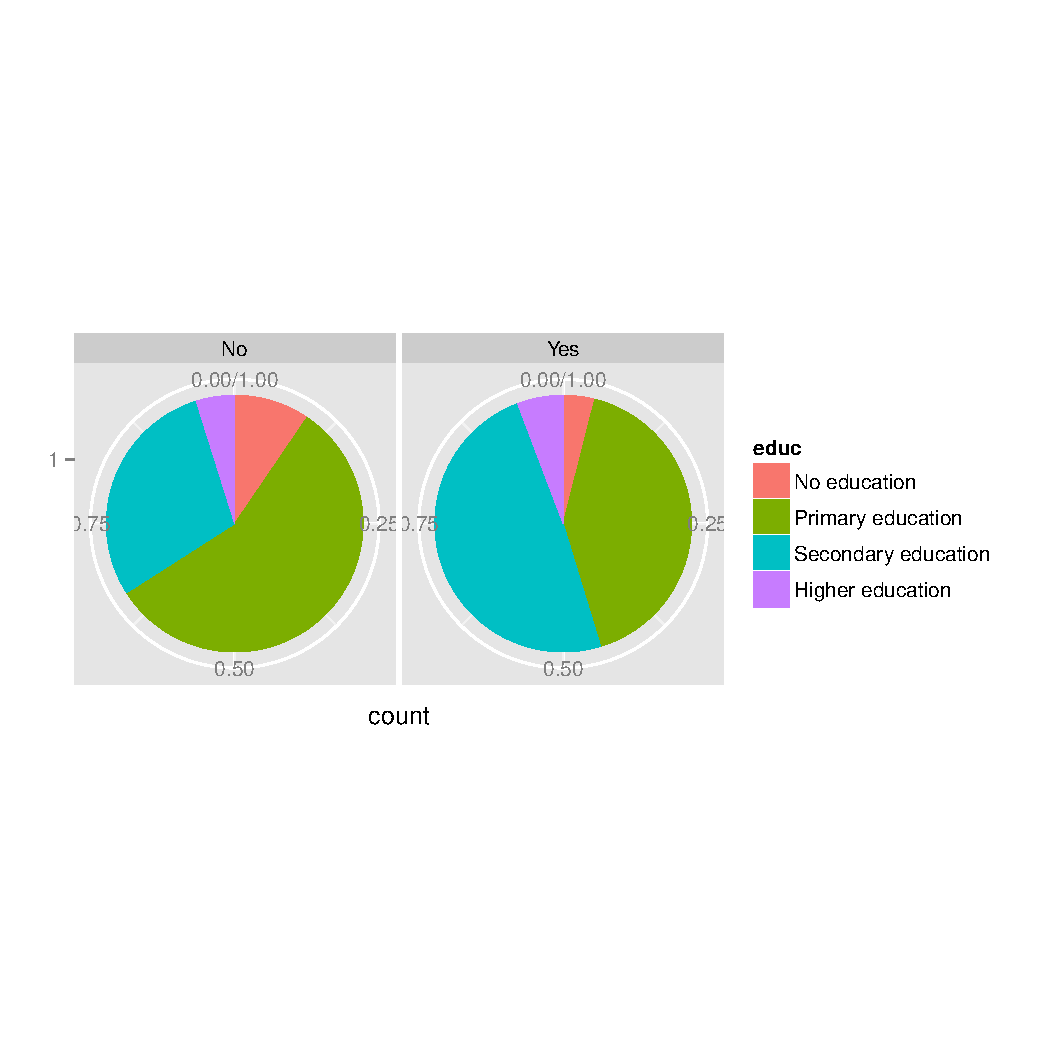
\includegraphics[width=\maxwidth]{figure/unnamed-chunk-41} 
\begin{kframe}\begin{alltt}
\hlcom{# *WITH ALTERED CAPTION}
\hlkwd{ggplot}\hlstd{(zambia4[}\hlopt{!}\hlkwd{is.na}\hlstd{(zambia4}\hlopt{$}\hlstd{clastsex), ],} \hlkwd{aes}\hlstd{(}\hlkwc{x} \hlstd{=} \hlkwd{factor}\hlstd{(}\hlnum{1}\hlstd{),} \hlkwc{fill} \hlstd{= educ,}
    \hlkwc{weight} \hlstd{= weight))} \hlopt{+} \hlkwd{coord_polar}\hlstd{(}\hlkwc{theta} \hlstd{=} \hlstr{"y"}\hlstd{)} \hlopt{+} \hlkwd{scale_x_discrete}\hlstd{(}\hlstr{""}\hlstd{)} \hlopt{+} \hlkwd{facet_grid}\hlstd{(}\hlkwc{facets} \hlstd{= .} \hlopt{~}
    \hlstd{clastsex)} \hlopt{+} \hlkwd{geom_bar}\hlstd{(}\hlkwc{width} \hlstd{=} \hlnum{1}\hlstd{,} \hlkwc{position} \hlstd{=} \hlstr{"fill"}\hlstd{)} \hlopt{+} \hlkwd{ggtitle}\hlstd{(}\hlstr{"Educational level of women by condom use at last sex"}\hlstd{)} \hlopt{+}
    \hlkwd{theme}\hlstd{(}\hlkwc{plot.title} \hlstd{=} \hlkwd{element_text}\hlstd{(}\hlkwc{vjust} \hlstd{=} \hlopt{-}\hlnum{30}\hlstd{))}
\end{alltt}
\end{kframe}
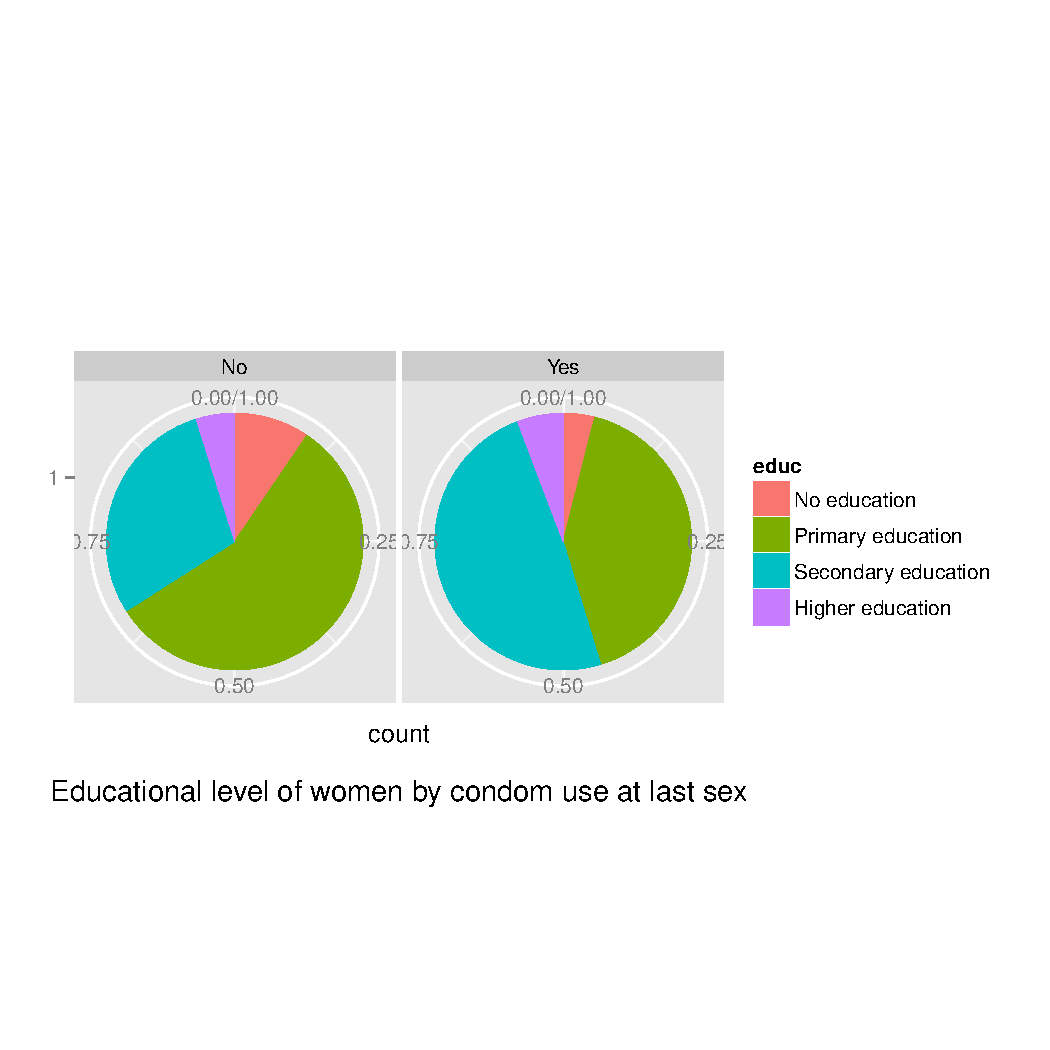
\includegraphics[width=\maxwidth]{figure/unnamed-chunk-42} 

\end{knitrout}

\end{document}
